\section{Architettura generale}
In questo capitolo verrà illustrata l'architettura generale di un sistema di IR e verranno
descritti alcuni processi che sono stati oggetto di studio del tirocinio.
Quando si parla di sistema di IR, oppure in termini più quotidiani di \textit{search engine},
siamo spesso abituati a vederlo come un sistema di interrogazione dove l'utente
digita come input un testo, chiamato query e il motore risponde con una serie di risultati. Tali risultati
sono visualizzati all'utente come una lista di documenti che contengono informazioni
rilevanti secondo la query.
\`E immediato pensare all'esempio di Google, dove l'utente digita una serie di termini
all'interno del  form e dopo qualche secondo gli vengono restituiti tutti i link a pagine web che
sono in qualche modo collegate a ciò che l'utente stava realmente cercando.
Quello che sta dietro a tutto questo processo, che sembra essere quasi immediato nell'esempio di Google, è
in realtà un lavoro molto complesso e lungo.
La fase che l'utente è abituato ad esserne partecipe è la fase finale, ovvero
il \textit{Retrieving}. Ma prima di poter parlare di ciò è necessario illustrare la fase primaria, l'\textit{Indexing}.

\paragraph{Alcune definizioni}
Per essere più chiari, conveniamo alcune definizioni di termini tecnici che al giorno d'oggi possono essere attribuiti
a concetti diversi.

\begin{definizione}\label{def:token}
	Un token è un'istanza di una sequenza di caratteri, in un documento $d \in \mathcal{D}$, che
	sono raggruppati tra di loro come un'unità semanticalmente utile.
\end{definizione}

\begin{esempio}[tokenizzazione]
	Nella frase "Nulla si crea, nulla si distrugge ma tutto si trasforma" i token sono i seguenti:
	\tokenbox{nulla} \tokenbox{si} \tokenbox{crea} \tokenbox{nulla} \tokenbox{si} \tokenbox{distrugge}
	\tokenbox{ma} \tokenbox{tutto} \tokenbox{si} \tokenbox{trasforma}.
\end{esempio}

Un altro concetto importante è il concetto di tipo.
\begin{definizione}[tipo]\label{def:tipo}
	Un tipo è una classe di token con la solita sequenza di caratteri.
\end{definizione}
\begin{esempio}
	Consideriamo la frase dell'esempio precedente. I tipi sono 7, mentre i token sono 10. Abbiamo dunque
	3 token che si ripetono.
\end{esempio}
\begin{definizione}[query]\label{def:query}
	Una query è un multinsieme di token, che rappresenta l'input che il motore di ricerca
	riceve dall'utente. 
\end{definizione}
Da notare che il concetto di multinsieme deriva dal fatto che si vuole tenere traccia in modo esplicito 
della molteplicità
dei termini nella query stessa.

\begin{definizione}[termine]\label{def:temine}
	Un termine è un tipo di una query.
\end{definizione}

\paragraph{Fase di indexing}
Per poter offrire quella velocità che si richiede durante la fase di retrieving è necessario aver ``preparato"
una struttura dati che sia completa, ovvero che comprenda tutte le informazioni necessarie, e 
rapida da scorrere, ovvero che le informazioni che si stanno cercando devono poter essere recuperate
il prima possibile.  Un esempio abbastanza esplicativo è quello dell'addetto alla biblioteca che deve rispondere
alle richieste degli studenti. Se l'addetto non conoscesse i libri che sono parte della biblioteca, per ogni richiesta
dovrebbe scorrere tutta la lista e capire se quel dato libro può essere utile oppure no.
Questo esempio rappresenta il fatto che l'addetto non è in possesso di una struttura in grado
di accedere solo alle informazioni necessarie ed è dunque inefficiente.
Se quindi non ci fosse un indice, per un motore di ricerca sarebbe troppo dispendioso elaborare tutti
i documenti "su richiesta".
La fase di indexing ha lo scopo di costruire una struttura dati, chiamata indice, che consenta
di velocizzare la fase successiva, il Retrieving.
Dal punto di vista delle prestazioni tale fase è quella con il  dispendio computazionale
più elevato, sia in termini di spazio che di tempo.
Questo perché si devono analizzare tutti i documenti della collezione ed eseguire una serie di elaborazioni
su di essi.
Il seguente algoritmo illustra in modo abbastanza basico ma intuitivo, la funzione eseguita dall'indexer.
\begin{algorithm}[h]
	\small
	\DontPrintSemicolon
	\SetKwInOut{Input}{Input}
	\SetKwInOut{Output}{Output}
	\Input{$\mathcal{D} $ collezione di documenti}
	\Output{$\mathcal{I}$ indice}
	\BlankLine
	$\mathcal{I} = generateEmptyIndex()$\;
	\ForEach{$d \in \mathcal{D}$}{
		$tokenizer = getTokenizer(d)$\;
		\While{$token = tokenizer.nextToken()$}{
			$n = normalizeToken(token)$\;
			$updateIndex(\mathcal{I}, n, d)$\;
		}
	}
	\Return{$\mathcal{I}$}
	\caption{\textsc{}}
	\label{alg:indexing}
\end{algorithm}
L'idea alla base è quella di rappresentare un documento come un flusso di token, il che è sempre possibile
poiché conveniamo che in questo campo di information retrieval i documenti sono solo di tipo testuale.
Il token prima di essere passato alla funzione $updateIndex$ viene normalizzato. La normalizzazione è un processo
che si occupa di risolvere alcuni problemi legati al riconoscere quando due token sintanticamente diversi
hanno invece la solita semantica\footnote{Potrebbe essere necessario uno step in più per risolvere il problema della codifica, poiché alcune lingue posseggono caratteri che non tutte le codifiche hanno. Per esempio le
lingue cirillica e cinese.}
Tale processo può essere schematizzato nel seguente modo, dove a sinistra viene indicato
il nome della normalizzazione e a destra una breve descrizione.
\begin{itemize}
	\item[Casing] le lettere maiuscole vengono convertite in minuscole
	\item[Accenti] le parole con accenti vengono convertite in parole senza accenti
	\item[Stemming] i verbi vengono convertiti in una forma normale, per esempio nel tempo infinito.
	\item[Lemmization] le parole plurali vengono convertite in singolari
\end{itemize}

\begin{esempio}[normalization]
	Sia data la seguente frase: ``\textit{Mi piacciono tutte le auto che sono elettriche}".
	Utilizzando le tecniche elencate in precedenza, i token normalizzati risultano:
	\tokenbox{Mi} \tokenbox{piacere} \tokenbox{tutte} \tokenbox{le} \tokenbox{auto}
	\tokenbox{che} \tokenbox{essere} \tokenbox{elettriche}.
\end{esempio}

\subparagraph{Indice invertito}
Una volta normalizzato si procede all'aggiornamento dell'indice, ovvero alla costruzione (o aggiornamento)
dell'indice invertito. Tale struttura è definita come una lista di coppie
$\langle token, PostingList \rangle$ dove PostingList è una lista di \textit{identificatori di documenti}.
In questo modo possiamo sapere il token $x$ in quali documenti è contenuto, cercando dentro l'indice
invertito la posizione di $x$ e accedendo alla sua \textit{postingList}.

\begin{figure}[h]
	\label{fig:invertedIndex}
	\centering
	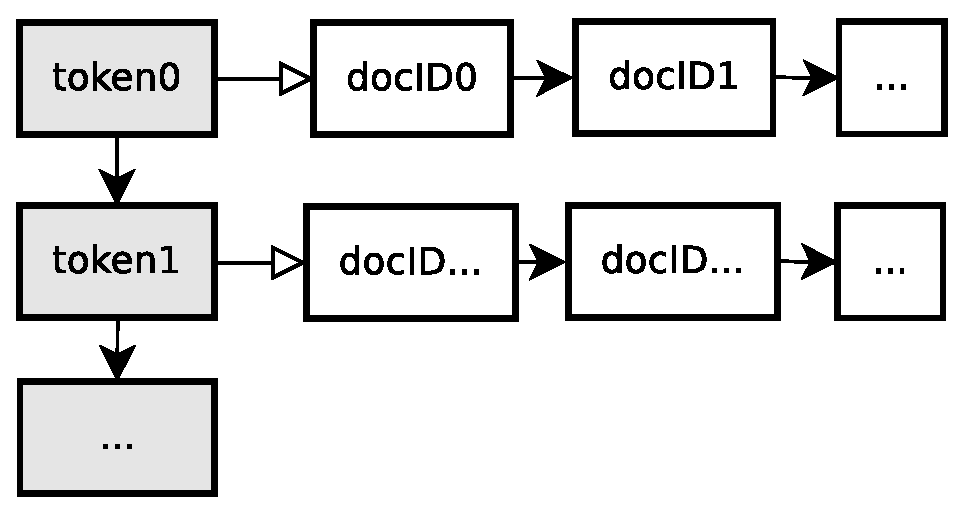
\includegraphics[scale=0.4]{InvertedIndex.eps}
\end{figure}

Ritornando all'esempio della biblioteca, se l'addetto avesse a disposizione l'indice invertito potrebbe:
\begin{enumerate}
	\item Raccogliere la query $\mathcal{Q}$ dello studente
	\item Normalizzare $\mathcal{Q}$
	\item $\forall t.t\in Q$ cercare all'interno dell'indice invertito il termine $t$ e \textit{ritornare} la \textit{postingList} associata
\end{enumerate}

In questo modo tutti i documenti che contengono almeno una volta un termine della query verrebbero mostrati
agli studenti, ma ovviamente non tutti possono essere rilevanti per la ricerca. Il problema dunque si ridotto
a come utilizzare l'indice invertito per capire quanto la query sia associata al documento in questione, ed è per questo
motivo che viene introdotta la fase di \textit{Retrieve}

\paragraph{Fase di Retrieving}
Lo scopo della fase di retrieving è quello di utilizzare l'indice invertito e affinare il modo con cui
i documenti vengono proposti all'utente, comunemente chiamati \textit{risultati}.
Tale processo prende anche il nome di ranking, poiché l'idea alla base è quella di attribuire
un punteggio ad ogni risultato e costruire una lista ordinata in senso crescente.
Ovviamente il primo risultato è quello secondo cui il sistema di ranking è più
rilevante per la query $q$. Tale processo viene fatto ogni volta che l'utente
interroga il sistema, per cui deve essere veloce, efficiente ed effettivo.
L'articolo \cite{10.1016/j.ipm.2016.05.004} mostra una serie di tecniche che possono essere
utilizzate per valutare il tradeoff tra qualità di un ranker ed efficienza, di cui alcune
sono state utilizzate nell'ambito di questo tirocinio.\\
Per essere più precisi possibile, possiamo definire la funzione di score nel seguente modo

\begin{definizione}\label{def:funzione_di_score_ideale}
	 Una funzione di scoring $f(d,q) : \mathcal{D} \times \mathcal{Q} \rightarrow \mathbb{R}$ è tale
	 se e solo se:
	 \begin{itemize}
	 	\item $f(d_1,q_1) \geq f(d_2, q_2) \implies rel(d_1, q_1) \geq rel(d_2, q_2)$,\\ dove $rel(d,q)$ è la rilevanza del documento $d$ per la query $q$, calcolata a priori.
	 	\item $f(d,q) \leq 0$ significa che il documento è irrilevante per $q$.
	 \end{itemize}
\end{definizione}

Tale definizione definisce una funzione di scoring ideale, per la quale non esiste un algoritmo che
la calcoli. Possiamo però accontentarci di funzioni che la approssimano, facendo uso di euristiche basate sulla statistica. \footnote{Solo per revisione: questo è quello che grossomodo credo di aver elaborato e penso che abbia anche una corrispondenza a livello teorico. }
Nei prossimi capitoli verranno descritte le funzioni di scoring che propongono BM25 e BM25P, le quali si basano sul concetto di \textit{Term Frequency} e \textit{Inverse Document Frequency}.
Prima di concludere la visione generale diamo la definizione di alcuni concetti che sono utilizzati durante il retrieving.

\begin{definizione}[Raw Count]\label{def:raw_count}
	$rc(q, D) : \mathcal{Q} \times \mathcal{D} \rightarrow \mathbb{N}$ è detto raw count, cioè il numero di volte che
	il termine q occore nel documento $d$.
\end{definizione}

\begin{definizione}[Term Frequency]\label{def:}
	La funzione $tf(q,d)$, acronimo di Term Frequency, è una funzione che calcola la frequenza del
	termine $q \in \mathcal{Q}$ nel documento $d \in \mathcal{D}$.
	Tale valore si discosta da quello di $rc$, poiché solitamente è normalizzato o in scala logaritmica
	oppure in base alla lunghezza del documento.
	
	\begin{itemize}
		\item $tf(q,d) = \log_{k>1}(1+rc(q,d))$
		\item $tf(q,d) = \frac{rc(q,d)}{|d|}$ dove $|d|$ è il numero totali di token nel documento
	\end{itemize}
\end{definizione}

\begin{definizione}[Inverse Document Frequency]\label{def:idf}
	$$
	idf(q, \mathcal{D}) = \log_{k>1}{
		\frac{\#\mathcal{D}}{
			\#
			\left\{
			d \in \mathcal{D} \middle \lvert rc(q,d) > 0
			\right\} 
		}
	}
	$$
	
	Tale misura esprime quanta informazione una parola, o più un generale un token, fornisce.
	Si può anche pensare come la misura dalla rarità, cioè quanto è comune il termine $q$
	nella collezione di documenti $\mathcal{D}$.
\end{definizione}




